\chapter{Synthesis}
\label{chapter:synthesis}

\section{Synthesizing rewrite rules for the simplifier TRS}

\section{Increasing Completeness: Synthesizing Rewrite Rules}
\label{sec:completeness}
%\jln{Possible TODO: I refer to expressions from the corpus we learn from as input expressions throughout. If anyone has a 
%better suggestion please let me know.}
\begin{figure*}
%\includegraphics[width=1.\columnwidth,natwidth=610,natheight=642]{figures/synthesis-flow.pdf}
%\includegraphics[width=1.\columnwidth]{figures/synthesis-flow.pdf}

% x_1 < select(x_2, c_0, c_1) + x_1 -> !x_2

  \tikzstyle{stage}=[fill=blue!10, draw=none, minimum height=3em, minimum width=11em]
  \tikzstyle{example}=[fill=orange!10, draw=none, minimum height=3em, minimum width=23em]
  \tikzstyle{label}=[fill=blue!10, draw=none, minimum height=3em, minimum width=1em]
  \begin{tikzpicture}[node distance=1.5cm,auto,>=latex']
    \node (s1) [stage] {\shortstack{Input expression}};
    \node (s2) [stage] [below of=s1] {\shortstack{Generated LHS\\patterns (Fig.~\ref{fig:lhspatterns})}};
    \node (s3) [stage] [below of=s2] {\shortstack{AC matching\\(Sec.~\ref{sec:rhsacmatching})}};
    \node (s4) [stage] [below of=s3] {\shortstack{Superoptimized with\\CEGIS (Sec.~\ref{sec:rhssynthesis})}};
    \node (s5) [stage] [below of=s4] {\shortstack{With symbolic\\constants (Sec.~\ref{sec:generalizing-constants})}};
    \node (s6) [stage] [below of=s5] {\shortstack{Substitute concrete\\values of $x_i$}};
    \node (s7) [stage] [below of=s6] {Candidate predicate};
    \node (s8) [stage] [below of=s7] {\shortstack{Verify or find new\\counterexample}};
    \node (s9) [stage] [below of=s8] {Rule with predicate};
    \node (s10) [stage] [below of=s9] {Add variants (Sec.~\ref{sec:filtering})};
    \node (l1) [label] [left of=s1,node distance=6em] {(a)};
    \node (l2) [label] [left of=s2,node distance=6em] {(b)};
    \node (l3) [label] [left of=s3,node distance=6em] {(c)};
    \node (l4) [label] [left of=s4,node distance=6em] {(d)};
    \node (l5) [label] [left of=s5,node distance=6em] {(e)};
    \node (l6) [label] [left of=s6,node distance=6em] {(f)};
    \node (l7) [label] [left of=s7,node distance=6em] {(g)};
    \node (l8) [label] [left of=s8,node distance=6em] {(h)};
    \node (l9) [label] [left of=s9,node distance=6em] {(i)};
    \node (l10) [label] [left of=s10,node distance=6em] {(j)};    

    \draw [line join=miter] (l8.west) -- ([xshift=-1em] l8.west) -- ([xshift=-1em] l6.west) -- ([xshift=-0.9em] l6.west) node {};
    \path[->] ([xshift=-1em] l6.west) edge node {} (l6.west);
        
    \path[->] (s1) edge node {} (s2);
    \path[->] (s2) edge node {} (s3);
    \path[->] (s3) edge node {} (s4);
    \path[->] (s4) edge node {} (s5);
    \path[->] (s5) edge node {} (s6);
    \path[->] (s6) edge node {} (s7);
    \path[->] (s7) edge node {} (s8);
    \path[->] (s8) edge node {} (s9);
    \path[->] (s9) edge node {} (s10);                

    \node (e1) [example] [right of=s1,node distance=19em]
          {$(y + 2) < \hsel(u < z, -3, 4) + (y + 2)$};
    \node (e2) [example] [right of=s2,node distance=19em]
          {\shortstack{
              \color{darkgray}
              \tiny{$\ldots$} \\
              \color{darkgray}
              \tiny{$(x_1 + 2) < x_2 + (x_1 + 2)$} \\
              $x_1 < \hsel(x_2, -3, 4) + x_1$ \\
              \color{darkgray}
              \tiny{$\hsel(x_1 < x_2, -3, 4)$} \\
              \color{darkgray}
              \tiny{$\ldots$}}};
    \node (e3) [example] [right of=s3,node distance=19em]
          {\shortstack{No reassociated/commuted variants \\ match an existing rule.}};
    \node (e4) [example] [right of=s4,node distance=19em]
          {$x_1 < \hsel(x_2, -3, 4) + x_1 \rightarrow \boxed{\neg x_2}$};
    \node (e5) [example] [right of=s5,node distance=19em]
          {$x_1 < \hsel(x_2, c_0, c_1) + x_1 \rewrites \neg x_2$};
    \node (e6) [example] [right of=s6,node distance=19em]
          {\shortstack{
              $0 < \hsel(\textit{false}, c_0, c_1) + 0 = \neg \textit{false} ~ \wedge$ \\
              $1 < \hsel(\textit{false}, c_0, c_1) + 1 = \neg \textit{false} ~ \wedge$ \\
              $0 < \hsel(true, c_0, c_1) + 0 = \neg true$ 
          }};
    \node (e7) [example] [right of=s7,node distance=19em]
        {$0 < c_1 \wedge c_0 \le 0 $};
    \node (e8) [example] [right of=s8,node distance=19em]
        {\shortstack{
            $\exists~ x_1, x_2, c_0, c_1 \;.\; (0 < c_1 \wedge c_0 \le 0) ~\wedge$ \\
            $(x_1 < \hsel(x_2, c_0, c_1) + x_1 \neq \neg x_2)$ ? \\
            No solutions. Predicate is sufficient.
        }};
    \node (e9) [example] [right of=s9,node distance=19em]
          {$x_1 < \hsel(x_2, c_0, c_1) + x_1 \rewrites \neg x_2 \pred 0 < c_1 \wedge c_0 \le 0 $};
    \node (e10) [example] [right of=s10,node distance=19em]
          {\shortstack{
              $x_1 < \hsel(x_2, c_0, c_1) + x_1 \rewrites \neg x_2 \pred 0 < c_1 \wedge c_0 \le 0 $ \\
              $x_1 < x_1 + \hsel(x_2, c_0, c_1) \rewrites \neg x_2 \pred 0 < c_1 \wedge c_0 \le 0 $
          }};



    \path[->] (e1) edge node {} (e2);
    \path[->] (e2) edge node {} (e3);
    \path[->] (e3) edge node {} (e4);
    \path[->] (e4) edge node {} (e5);
    \path[->] (e5) edge node {} (e6);
    \path[->] (e6) edge node {} (e7);
    \path[->] (e7) edge node {} (e8);
    \path[->] (e8) edge node {} (e9);
    \path[->] (e9) edge node {} (e10);

  \end{tikzpicture}
  \caption{Overall flow of the synthesis pipeline (in blue) with worked example (in orange). (a) We harvest expressions from real compilations on which the TRS could make no further progress. (b) We enumerate all subtrees of these to generate left-hand sides that would match each expression. Our example will focus on one such pattern. (c) We obtain a right-hand side by first checking if any reassociated or commuted variants of it match an existing TRS rule. (d) If not, we superoptimize the pattern using CEGIS. (e) This rule is specific to the particular values of any constants that appear. We then replace any constants with new variables $c_0, c_1, etc.$, to obtain a more general version of the rule. We must now synthesize a sufficient condition on these new variables under which the rule still holds. (f) To do this, we treat the rewrite as an equality and take the conjunction over a set $S$ of different values for the non-constant variables $x_0, x_1, etc.$ (g) Simplifying the result gives a candidate predicate. This is a \emph{necessary} condition. (h) We then check if it is also \emph{sufficient} condition using Z3. (i) If a counterexample is found, we add these new values of $x$ to $S$ to obtain a new candidate predicate and repeat until we have a sufficient condition to serve as our predicate. (j) Finally, we construct variants of the rule in which the LHS has been commuted.}
\label{fig:synthesis-flow}
\end{figure*}


Although the Halide term rewriting system is necessarily incomplete, we can strengthen 
it by finding expressions on which the TRS can no longer make progress and creating 
rules that will further simplify them.
In this section, we describe a workflow for automatically augmenting the Halide TRS with new rules.

Given an \emph{input expression} that the TRS failed to simplify, our goal is to find a rule that
can rewrite it. A high-level view of the synthesis pipeline is shown in Figure~\ref{fig:synthesis-flow}.
%and Algorithm~\ref{alg:synthesis-algorithm} shows the corresponding pseudocode.
We begin with an expression we will attempt to further simplify; 
first, we synthesize rules that contain concrete constants from the input expression. 
Next we generalize those rules by replacing constant values with symbolic constants and synthesizing compile-time 
predicate guards 
that check the validity of the rule on the values matched by the symbolic constants. If we 
find such a rule, we know that adding it to the TRS will enable it to simplify the input
expression as well as any similar expressions it may encounter.

The set of input expressions may come from a bug report, or may be gathered from compiler logs. With logging enabled, the compiler records two
kinds of problematic expression for which new TRS rules may be helpful:
non-monotonic expressions, which can result in over-conservative
bounds for loops and memory allocations; and proof failures,
which may prevent Halide from performing certain optimizations
(see Section~\ref{sec:uses-of-trs}). 
Of course, absent an oracle, it is difficult to know if the TRS has fully simplified 
some expression or if it lacks the solving power to continue simplification. 
When the TRS is used as a proof engine, its goal is to reduce an expression to true.
In this case, we can fuzz-test failed proofs by assigning all variables in an expression
random values and evaluating; if we cannot find an assignment that evaluates to false,
the expression may indeed be reducible to true, so we log it as an input expression.


\begin{figure*}
\begin{tabular}{lll}
\begin{tikzpicture}[level distance=12mm,baseline=(current bounding box.center)]
\tikzstyle{level 1}=[sibling distance=15mm]
\tikzstyle{level 2}=[sibling distance=8mm]
\tikzstyle{level 3}=[level distance=10mm,sibling distance=5mm]

% tried to label subtrees but positioning looks weird, fix later
\node (+) {+}
  child { node (+2) {+}
    child { node (z) {z}  } % edge from parent node[left,draw=none] {$v_1$}
    child { node (2) {2} }}
  child { node (min) {\hmin}
    child { node (x) {x}}
    child { node (-) {-} %edge from parent node[right,draw=none] {$v_2$}
      child {node (y) {y}}
      child {node (z1) {z} } % edge from parent node[right,draw=none] {$v_3$}}
    }};


\begin{pgfonlayer}{background}
\fill[red,opacity=0.3] \convexpath{x, min, z1, y}{10pt};
\fill[blue,opacity=0.3] \convexpath{y, -, z1}{10pt};
\fill[green,opacity=0.3] \convexpath{z, +2, 2}{10pt};
\end{pgfonlayer}
\end{tikzpicture} &
\begin{tabular}{llll}
$(z + 2) + \hmin(x, y - z)$ & $\hmin(x, y - z)$ & $z + 2$ & $y - z$ \\
$v_1 + \hmin(x, y - z)$ & $\hmin(x, v_2)$ & & \\
$v_1 + \hmin(x, v_3)$ & & & \\
$(z + 2) + \hmin(x, v_3)$ & & & \\
$v_1 + v_2$ & & &
\end{tabular}
\end{tabular}
\caption{Given the input expression $(z + 2) + \hmin(x, y - z)$, we find all possible 
LHS patterns by substituting fresh variables for subterms, for all valid combinations. Then, we repeat the process for 
each individual subterm. This process yields the list of candidate LHS terms on the right.}
\label{fig:lhspatterns}
\end{figure*}

\subsection{Generating LHS Patterns}

  Our first step is to find LHS terms that could match the input expression, or any portion of it. 
We can enumerate all such terms through a kind of inverse matching.
When we rewrite an expression with a rule, 
we match the expression to the rule's LHS by finding a substitution for all variables in
the LHS that will unify it with the input expression. Here, we start with an input expression,
then fix a substitution by mapping some of its subterms to fresh variables. We 
replace those subterms with the new variables, constructing a term that can 
be matched with the input term.
If we perform this inverse matching for all sets of subterms, we find \emph{all possible LHSs} that could match the
input expression. 
When a subterm occurs more than once in the input expression, we construct a LHS that 
uses the same variable to replace it in multiple places and LHSs that replace its
occurrences with different variables.
We repeat the procedure on all \emph{subterms} of the input expression.  The result is the set of all 
LHSs that match any part of the input expression. See Figure~\ref{fig:lhspatterns} for a worked example.

This number of LHSs is exponential in the size of the input expression, so we use a few heuristics to narrow 
our search. We bound the size of candidate LHSs to have seven or fewer leaves, since longer terms are less likely to 
result in rules general enough to justify inclusion in the ruleset. 
Additionally, since we process input expressions in batches, we remove 
duplicate LHSs as well as LHSs that differ only in the values of their constants. 
Finally, we have found it helpful to keep a blacklist of LHSs for which we previously
failed synthesize rules; for example, $v_1 + v_3$ 
cannot form a rule, so we filter it out as a candidate.

\subsection{Synthesizing Right-Hand Sides} 
\label{sec:synthesizing-candidate-rules}
%
Given a candidate left-hand side, we attempt to 
synthesize a right-hand side that is semantically equivalent and
respects the reduction order, namely $\mathit{LHS} > \mathit{RHS}$.
We employ two strategies for synthesizing right-hand sides:
delayed AC matching, and counter-example guided inductive synthesis (CEGIS) of 
the RHS followed by synthesis of the rule predicate guard.

\subsubsection{Finding Right-Hand Sides through AC Matching}
\label{sec:rhsacmatching}
The first strategy reflects the Halide design decision not to perform any AC matching in the TRS, for efficiency reasons. 
Instead, AC matching is effectively performed during rule synthesis, by checking whether the LHS could be 
rewritten by the existing TRS after a suitable application of associativity and commutativity laws to the LHS. 
To this end, we generate all possible reassociations and commutations of the candidate LHS term and pass them to the existing TRS. 
If any of them can be simplified, we create a new rule that rewrites 
the original, untransformed LHS term to the result of the simplification.  Note that this result may include applications of more than one rewriting step, so the new rule is not merely an AC-variant of an existing rule.

For example, assume our TRS includes the rule $(x + y) - x \rewrites y$, 
and let $((u + 2) + v) - u$ be a candidate LHS term. The rule does not match the candidate but it matches its variant $(u + (v + 2)) - u$, rewriting it to the result $v + 2$. The candidate and the result give us the rule $((u + 2) + v) - u \rewrites v + 2$.

We can consider this procedure a kind of lazy offline AC matching, because if the Halide TRS 
performed full AC matching while rewriting expressions, it would be able to apply the rule $(x + y) - x \rewrites  y$ to the candidate expression $((u + 2) + v) - u$ after reassociating it to $(u + (v + 2)) - u$, obtaining the result $v + 2$.  Delaying AC matching to synthesis has the effect of restricting the system to a single, offline round of AC and memoizing the result in the form of a new TRS rule if we are successful. 
Note that the synthesis procedure below could have found this rule, but checking for AC
variants of existing rules is far cheaper. About three-quarters of our synthesized rules are generated by this method.

\subsubsection{Finding Right-Hand Sides through CEGIS}
\label{sec:rhssynthesis}
If the first method fails, we apply counterexample guided inductive synthesis (CEGIS)~\cite{DBLP:conf/aplas/Solar-Lezama09} to superoptimize the left-hand side pattern.
In superoptimization~\cite{massalin1987superoptimizer}, we take a program and search 
for an equivalent program within some grammar that is preferable according 
to some cost function. Here our grammar is that of the Halide expression language, 
the method for testing program equivalence is the Z3 solver, and we use the node
count of the programs as a proxy for our full reduction order.

Similar to prior work in superoptimization~\cite{regehr2018superoptimization, mangpo2016superoptimization},
we search the expression space for an equivalent RHS using a CEGIS loop. This loop alternately calls Z3 as a
verifier, which checks if a candidate RHS is equivalent to the LHS on all inputs, 
and a learner, which finds a candidate RHS that is equivalent to the LHS on
a limited set of inputs.
We begin by choosing a single-op
RHS and ask the verifier if it is equivalent to the LHS. If it is not, we get back 
a counterexample of assignments to the variables for which the right- and left-hand side are 
not equivalent, which we keep as a set of test inputs. 
We then ask the learner for a new RHS that is equivalent to the LHS 
only on the counterexample assignments we found in the last step. 
If we cannot find an equivalent single-op sequence,
we iteratively increase the number of operations, ensuring we find shorter sequences
first.  If CEGIS returns a sequence semantically equivalent to the LHS pattern with fewer
operations, we use it together with our LHS to form a candidate rule.

 The learner portion of the CEGIS loop creates a candidate RHS
  %expression from a parameterized bytecode
  %sequence of fixed size that is fed to an interpreter. Each bytecode
  %instruction takes parameters that select between the possible operators and
  %operands available to it. Thus,
  %this bytecode
  %sequence serves as an SSA representation of an expression tree. The
  %interpreter is evaluated abstractly on symbolic inputs to produce a
  %sketch~\cite{DBLP:conf/aplas/Solar-Lezama09, torlak2014lightweight}, 
  %capable of acting as any Halide expression in our
  %search space depending on the bytecode values. The learner uses Z3
  by creating a sketch~\cite{DBLP:conf/aplas/Solar-Lezama09, torlak2014lightweight}
  that consists of a small bytecode interpreter that encodes the possible
  operations and operands the RHS can use, along with a bound on the number of instructions.
  The learner uses Z3 to query for a sequence of bytecodes within the bound, that, when
  run through the interpreter, is semantically
  %solve for the bytecode values that makes the sketch semantically
  equivalent to the LHS over the test inputs. If a solution is found,
  substituting the produced bytecode values into the sketch
  and applying the TRS reduces it to a concrete candidate RHS. One
  complication arising from this approach is that a bytecode sequence
  of a fixed number of ops may produce expression trees of a larger
  size if intermediate values are reused. We reject any such solutions
  in a post-pass by checking each synthesized RHS against the LHS
  using the full reduction order. An alternative solution would be
  introducing let bindings into our search space so that the size of
  the expression tree could be bounded by the number of ops in its SSA
  form. However, we could not identify any significant rewrite rules
  lost to this filtering, so we deemed this an unnecessary
  complication. 

While Z3 is a powerful tool for synthesis, there are certain types of expressions 
containing division or modulo that Z3 nearly always fails to reason about during the CEGIS process. (We experimented with the SMT solvers Yices2~\cite{jovanovic2017solving} and MathSAT5~\cite{mathsat5}, but were not able to obtain appreciably better results.)
Z3 is better able to reason about expressions containing concrete constants, rather than
universally quantified variables, so we synthesize rules using candidate LHSs with 
concrete constants from the input expression and generalize them later.
We limit the use of division and modulo in our op-codes to be division
or modulo by 2 only, and rely on the generalization step described next to
widen the set of denominators for which a rule applies.  Because of this
restriction, our synthesized rules cannot contain non-constants in denominators
or the right-hand side of a modulo.  As a result, our synthesis system cannot
construct all rules a human can.

\begin{table*}
\caption{Sample rules synthesized by our process. }
\small
\begin{tabular}{l|l|l}
LHS & RHS & Predicate \\
\hline
$(x*y) - (z + (w*x))$ & $(x*(y - w)) - z $ & \\
$x < (y + x) + z$ &  $0 < (y + z)$ & \\
$\hmax(x*x, y) + \hmax(z, w*w) < c_0$ & false & $c_0 <= 0$ \\
$\hsel(x, c_0, y) < \hmin(\hsel(x, c_1, y), c_2)$ & false & $\hmin(c_1, c_2) <= c_0$ \\
$\hmin((x + ((y - x)/c_0)*c_0) + c_1, y)$ & $y$ & $1 <= c_1 \wedge -1 <= (-1/c_0)*c_0 + c_1$ \\
\end{tabular}
\label{tab:samplerules}
\end{table*}

\subsection{Generalizing Constants and Finding Predicate Guards}
\label{sec:generalizing-constants}

If either AC-matching search (Section~\ref{sec:rhsacmatching}) or CEGIS-based synthesis (Section~\ref{sec:rhssynthesis}) were successful, 
we now have a candidate rewrite
rule that contains concrete values originating from the input expression.
To generalize the rule, we replace such constants with fresh \emph{symbolic constants} 
and synthesize a guard that is true when the rule is valid. 
Recall that in the Halide TRS, a variable in the LHS matches any subterm, while a 
symbolic constant matches only a constant value (see Section~\ref{sec:customalgo}); the guards, which are predicates over symbolic constants, can thus be evaluated at compile time. 

Our goal is to generalize the equality by synthesizing a guard predicate $\phi$ 
over the symbolic constants in the LHS and RHS terms such that our rule is valid whenever
$\phi$ evaluates to true:
\[ \forall \vec{c} \forall \vec{x} \;.\; \phi(\vec{c}) \implies LHS(\vec{x},\vec{c}) = RHS(\vec{x},\vec{c})
\]

First, we check to see if this condition is satisfied when $\phi$ is 
always true. If it is, then no predicate guard is needed. Otherwise, we need 
to synthesize an expression for $\phi$. We find candidates for $\phi$ iteratively 
by first choosing a small set of values $S$ for the variables 
in $\vec{x}$ and finding the candidate guard $\phi_S$. We check to see if $\phi_S$
is a sufficient predicate guard for all $\vec{x}$; if it is not, we add
counterexamples to the set $S$ and repeat.

\[ \forall \vec{c} \forall \vec{x} \in S \;.\; \phi_S(\vec{c}) \implies LHS(\vec{x},\vec{c}) = RHS(\vec{x},\vec{c})
\]

We initialize $S$ with all basis vectors, which are 
values $\vec{x} = ( 0, \ldots, 0, 1, 0, \ldots, 0 )$ that include exactly one unit value,
plus the zero vector.  
We then unwind the right-hand side of the implication and substitute in the concrete values 
from $S$ to get:

\[ \forall \vec{c} \forall \vec{x} \in S \;.\; \phi_S(\vec{c}) \implies (LHS(\vec{x_1},\vec{c}) = RHS(\vec{x_1},\vec{c}) \wedge \ldots \wedge
LHS(\vec{x_k},\vec{c}) = RHS(\vec{x_k},\vec{c}))
\]

We use the Halide TRS itself to simplify the conjunction on the right-hand side of the
implication. Since all occurrences of $\vec{x}$ have been replaced with concrete
values, we get back an expression that contains only symbolic constants, which we
use as our candidate guard $\phi_S$.

We test whether $\phi_S$ is sound on all $\vec{x}$.
\[ \exists \vec{c} \; \exists \vec{x} 
   \;.\; LHS(\vec{x},\vec{c}) \not= RHS(\vec{x},\vec{c})
\]

If this query has a solution $\vec{x}$, then the guard is unsound.  
If so, we add the counterexample $\vec{x}$ to $S$, and construct a new guard $\phi_S$.  
We repeat this process for several iterations (four, in our experiments) and if 
we fail to find a sound guard, we switch to an alternative strategy that converts 
the current (unsound) candidate $\phi_S$ to disjunctive normal form and tests
each clause in turn to check if it is a sufficient guard.
If it is, that clause becomes the guard.  If no clause is sound, we discard the rule.
If the loop terminates with Z3 timing out or returning ``unknown'', we return
the current $\phi_S$, flagging it as requiring a manual proof. 
We exclude all such cases from our experiments.


As an example, consider the candidate rule:
%
\[ x_0 < \hsel(x_1, c_0, c_1) + x_0 \rewrites \neg x_1
\]
We initialize $S$ with three basis vectors $\{(0,\mathit{false}), (0,\mathit{true}), (1,\mathit{false})\}$ and construct $\phi_S$:
%
\begin{equation*}
\begin{split}
 \phi_S(\vec{c}) \iff 
 &  \forall_{\vec{x} \in S} \;.\; LHS(\vec{x},\vec{c}) = RHS(\vec{x},\vec{c}) \\
 \iff & 
 0 < \hsel(\mathit{false}, c_0, c_1) + 0 = \neg\mathit{false} \; \wedge \\
                                                   & 0 < \hsel(\mathit{true}, c_0, c_1) + 0 = \neg \mathit{true}  \; \wedge \\
                                                   & 1 < \hsel(\mathit{false}, c_0, c_1) + 1 = \neg\mathit{false}
\end{split}
\end{equation*}

Simplifying the RHS with the TRS, we obtain $\phi_S$:
%
\[  \phi_S(\vec{c}) \iff 0 < c_1 \wedge c_0 \le 0
\]

Next we check whether $\phi_S$ is sound for all $\vec{x}$.  It is, so we have a completed rule:

\[ x_0 < \hsel(x_1, c_0, c_1) + x_0) \rewrites \neg x_1 \;\pred \;0 < c_1 \wedge c_0 \le 0
\]


\subsection{Adding Rule Variants}
\label{sec:rulevariants}
Once we have a generalized rule with a valid predicate, we eagerly compensate for the lack
of AC matching in the Halide TRS by adding AC variants of the rule as well. We find 
all commuted variants of the rule's LHS,
with respect to the partial commutative canonicalization as described in Section~\ref{sec:customalgo}.
 (This is exponential in the size of the number 
of commutative operators, which is tractable given our bounds on LHS term size). 
Then, we find all reassociations of the rule's right-hand side. For each variant LHS, 
we choose a RHS variant by serializing expressions to strings and finding the RHS 
that has the shortest edit distance from that LHS.

For example, the LHS of the first rule below has four additions and can be commuted 
to 16 variants. The RHS of the rule can be reassociated in two different ways. For the 
commuted variant of the LHS on the second line, we choose the other means of reassociating
the RHS as it has a smaller edit distance.

\begin{equation*}
\begin{split}
(x + (y - ((z + (w + x)) + u))) & \rewrites y - (z + (w + u))) \\
(y - (((w + x) + z) + u)) + x & \rewrites y - ((z + w) + u)
\end{split}
\end{equation*}

The intuition is that there is no a priori reason 
to prefer one reassociated variant to another; they are almost certainly equal in 
terms of our reduction order. Thus, we choose the RHS that perturbs the structure of the 
LHS as little as possible, in order to avoid rewriting common subexpressions in the hopes
of canceling them out later.


\subsection{Filtering Rule Output}
\label{sec:filtering}
As a final step, we check each output rule for redundancy with the rule batch found
by the synthesis pipeline. For each new rule, we check
that no earlier rule has precisely the same LHS and predicate; if so, it can be discarded.
Then, we check that no earlier rule is more general than the current rule: a rule is more 
general than another if they have similar LHSs, but a variable appears in the first rule 
in a place where the second rule has a more specific subterm, or if they have the same LHS
but the predicate of the first rule implies the predicate of the second.

Finally, we
check that the candidate rule obeys our reduction order in order to
preserve our termination guarantee. If the candidate rule passes these
filters, and the predicate has not been flagged for human review, the
rule can be added to the TRS ruleset automatically without any human
auditing.

\section{Evaluation of Simplifier TRS Synthesis}

\section{Evaluation}
\label{sec:evaluation}

% (1186-367)/1186
\newcommand{\PercentPossibleToSynth}{69\%}
\newcommand{\NumRulesInCorrectnessExperiment}{321}
\newcommand{\PercentRulesResynthesized}{58\%}

In evaluating the benefits of the verifier and synthesizer, we answer the following questions:

\begin{itemize}
  \item \textbf{Does the synthesizer produce better rules than a human expert?} The TRS has been manually extended five times in response to bug reports pointing out limitations of the compiler. We synthesized these five rulesets automatically and found that the human-authored rules were less general and in one case were incorrect. (Section~\ref{sub:bugfixes})
 
  \item \textbf{What is the best way to use synthesis and verification in development?} We survey several cases from recent Halide development where human experts used the synthesis machinery as an assistant, finding that this hybrid model is more powerful than either the human developer or the synthesizer alone. (Section~\ref{sub:synthassistant})
  \item \textbf{Can synthesis be used for large-scale improvements of the TRS?} We gather a corpus of over 100,000 expressions on which the TRS can make no progress and iteratively synthesize rules using the corpus as input. We synthesize \NumRulesSynthesized  rules and add them to the TRS ruleset without a human audit. We find that the enhanced ruleset reduces peak memory usage in compiled code, sometimes dramatically, in 197 of our benchmarks. We also find no significant compile-time slowdown even with this 4.5-fold increase in ruleset size. (Section~\ref{sub:endtoendexperiment})
  \item \textbf{Could the entire TRS have been synthesized?} Encouraged by the large-scale experiment, we ask how far we are from being able to bootstrap the entire TRS automatically---something that we considered too ambitious originally. First, we find that \PercentPossibleToSynth~of the existing ruleset is accessible to our current synthesizer in principle; the remaining rules contain operators not yet supported by the tool. % or cannot be reasoned about automatically by our solver. 
  We test the synthesizer's power by removing \NumRulesInCorrectnessExperiment{} accessible rules from the original ruleset one by one and attempting to synthesize a replacement, successfully finding a replacement rule \PercentRulesResynthesized{} of the time.  We find this encouraging for future applications of the synthesizer. (Section~\ref{sub:replacementexperiment})
\end{itemize}

We discuss these findings in more detail below, grouping them into three sections. First we examine bug reports from Halide’s past and evaluate whether the machinery presented in this paper could have fixed them automatically. Second, we examine cases where beta versions of our verifier and synthesizer assisted humans both in fixing bugs and in correctly making larger changes to the compiler. Third, we fuzz the compiler to mine for issues that could be fixed with new simplifier rules, and automatically fix them before they ever appear as a bug in a real program. In this way we demonstrate that this machinery would have been useful in the past, is useful in the present, and will help avoid entire classes of bugs in the future.

%\jln{don't forget to do this!}
%Note for reviewers: For the purposes of this anonymous submission, we will refer to code changes by letter, with corresponding diffs found in supplemental material. In this final version of the paper these will be replaced with GitHub issue and pull request IDs with links to Halide’s GitHub page.

\subsection{Comparing the Synthesizer to Human-Authored Rules}

\subsubsection{Does the Synthesizer Produce Better Rules than a Human Expert?}
\label{sub:bugfixes}

%We expect a human expert to create rules that are as general as possible while also including rules that take advantage of less general situations, such as when special cases allow stronger rewrites.  Can a synthesizer produce rules that are both general and expressive? 

%We compared synthesized rules against five sets of rules added manually. We have found that the expert wrote rules that were less general than the synthesized rules, and in some cases were incorrect. Additionally, the synthesizer avoided adding a specialized rule because the TRS could already achieve its effect with rules present in the TRS. We discuss in Section~\ref{sec:limitations} the limitations of when the synthesizer cannot achieve such general rules. 

% AA: I found the two paragraphs above redundant with the summary we just gave in the itemized list.


% A) https://github.com/halide/Halide/pull/3719
% B) https://github.com/halide/Halide/pull/3761
% C) https://github.com/halide/Halide/pull/3765
% D) https://github.com/halide/Halide/pull/3770
% E) https://github.com/halide/Halide/pull/3780
% F) https://github.com/halide/Halide/pull/4721
% G) https://github.com/halide/Halide/pull/4772
% H) https://github.com/halide/Halide/pull/4439
% I) https://github.com/halide/Halide/pull/4850 


We searched through Halide’s change history and selected the five pull requests that addressed issues by adding new rewrite rules to Halide’s TRS. These pull requests occurred before the Halide developers started routinely using the verifier and synthesizer when changing the TRS. These can be found as summarized diffs $\mathbb{A}$-$\mathbb{E}$ in supplemental material, or in their original form on the Halide project website
\footnote{
$\mathbb{A}$: \url{https://github.com/halide/Halide/pull/3719}
$\mathbb{B}$: \url{https://github.com/halide/Halide/pull/3761}
$\mathbb{C}$: \url{https://github.com/halide/Halide/pull/3765}
$\mathbb{D}$: \url{https://github.com/halide/Halide/pull/3770}
$\mathbb{E}$: \url{https://github.com/halide/Halide/pull/3780}
}.
Creating these rewrite rules as a human is an amount of work disproportionate to the size of the change. The author of the rules must prove them correct on paper, and a second reviewer must check their work. As we will see, bugs can slip through despite this review. 

In each case we take the test expressions committed as part of the change and feed them to our synthesizer to see if it would have produced the same rewrite rules as the humans did. In cases where humans did not check in tests for their new rules, we wrote our own. In total, across these five cases humans added 24 new rules. The synthesizer generated 42, covering all but one of the human rules, while correcting and generalizing others. In cases $\mathbb{A}$, $\mathbb{C}$, and $\mathbb{E}$, the rules generated by the synthesizer are an exact match to the human-generated rules. In case $\mathbb{B}$ the synthesizer matched the human but also crafted 8 commuted variants of the human rules, making them more widely applicable. 
\newpage
As an example, for the human-written rule:

\[
\hmax(\hmax(x, y) + c_0, x) \rewrites \hmax(x, y + c_0) \pred c_0 < 0
\]

The synthesizer produced effectively the same rule, along with a variant:

\begin{align*}
& \hmax((\hmax(x, y) + c_0), x) \rewrites \hmax((y + c_0), x) \pred c_0 \leq 0 \\
& \hmax(x, (\hmax(x, y) + c_0)) \rewrites \hmax(x, (y + c_0)) \pred c_0 \leq 0
\end{align*}

Case $\mathbb{D}$ is the most interesting. It contains four rules involving comparisons of $\hmin$ and $\hmax$ operations. What happened for each was identical, so we will only discuss the $\hmin$ rules. The first rule is:

\[
\hmin(x, c_0) < \hmin(x, c_1) + c_2 \rewrites \hfalse \pred c_0 \geq c_1 + c_2)
\]

This rule is incorrect (consider $c_0 = c_2 = 1$, $x = c_1 = 0$). It can be fixed by adding the term $c_2 \leq 0$ to the predicate. The synthesizer produced the correct version of this rule, along with two generalizations of it:

\begin{align*}
& \hmin(x, c_0) < \hmin(x, c_1) + c_2 \rewrites  \hfalse \pred c_2 \leq 0 \wedge c_1 + c_2 \leq c_0 \\
& \hmin(x, c_0) < \hmin(x, y) + c_1 \rewrites c_0 - c_1 < \hmin(x, y) \pred c_1 \leq 0 \\
& \hmin(x, c_0) < \hmin(y, x) + c_1 \rewrites c_0 - c_1 < \hmin(y, x) \pred c_1 \leq 0
\end{align*}

The second human rule was:
\[
\hmin(x, c_0) < \hmin(x, c_1) \rewrites \hfalse \pred c_0 \geq c_1
\]
The synthesizer found a more general rule, along with three other commuted variants (elided for space):
\[
\hmin(x, y) < \hmin(x, z) \rewrites y < \hmin(x, z)
\]
Any expression which matches the human-written rule would also match the synthesized one. The synthesized version does not simplify to the constant false in a single step. However, after applying this rule to the case considered by the human, we get $c_0 < \hmin(x, c_1)$ where $c_0 \geq c_1$. The simplifier then reduces this to false in a second step, so the human-written rule becomes unnecessary. The synthesizer considered the human-written rule, but discarded it as less general than the one above.

Case $\mathbb{D}$ also included the rewrite rule: 
\[
x\; \%\; x \rewrites 0
\]
which was the sole rule the synthesizer could not generate, as we did not include modulo by non-constants in our CEGIS interpreter.

With this one exception, across these five code changes the synthesizer generated more general, more correct rules than the humans, and would clearly have been a useful assistant to the Halide developers if they had had it at the time.


\subsubsection{What Fraction of the Halide Rules Could Have Been Synthesized?}
\label{sub:replacementexperiment}
To bootstrap a TRS, we could start with a TRS equipped with a basic set of rules and synthesize the remaining rules as the TRS encounters expressions needing those rules.  How far is the synthesizer from supporting this ambitious vision?

Given the space of possible rewrites explored by the synthesizer, we believe that it can currently produce at most \PercentPossibleToSynth{} of rules that exist in the current TRS. The obstacles to synthesizing all human-written rules include (i)~the inability to automatically verify some rules or preconditions (see Question 3 above); and (ii)~lack of support for some operators in our synthesizer. 

We tested the synthesizer's ability to recreate the original ruleset in the following experiment. We instrumented the ruleset to associate expressions from compilations of Halide's correctness test suite with individual rules invoked when those expressions are rewritten. We gathered a set of rules for which we had at least three expressions that matched the rule, and filtered out those rules that are out of scope for the current synthesizer, because their right-hand sides contain operators we do not support. This gave us a set of \NumRulesInCorrectnessExperiment{} rules. For each of these rules, we disabled the rule in the TRS, then used its matching expressions as input to the synthesizer. The synthesizer was able to find rules in 186 cases, or about \PercentRulesResynthesized{} of the rules. Of the other 135 cases, in 43 of them other rules in the existing TRS happened to combine to rewrite the specific input expression even without the target rule; for example, this often occurred when the matching expression contained combinations of constants that could be exploited by other rules. 10 of the 92 failure cases were due to timeouts in the synthesis process, while 15 specifically failed to synthesize a predicate. Given that it was difficult to target the desired rule precisely, we find these results to be a promising state of the technology.


\subsection{Practical Uses of the Synthesizer and Verifier}





\subsubsection{What is the Best Way to Use Synthesis and Verification in Development?}
\label{sub:synthassistant}

% Is the expert equipped with the synthesizer better at developing rules than either the expert alone or the synthesizer alone? The synthesizer can accelerate rule development because it is correct by construction and also faster than a human expert. On average, the expert needed about 30 minutes to develop a rule, including a paper proof and the code review. Our synthesizer typically produces a batch of ten (verified) rules in about 5 minutes.

We have found that human experts can best leverage the strengths of the synthesis tool by using it as an assistant: for example by synthesizing a rule and then generalizing or simplifying it by hand, or by writing a rule and asking the tool to synthesize a valid predicate. Most importantly, this avoids committing new bugs, but it also accelerates rule development. Halide developers report that adding new rules by hand takes about 30 minutes per rule starting from sample input expressions through final review. Starting from the same input expressions, the synthesis tool can produce a batch of 10 verified rules in about 5 minutes.

Here we survey some cases from recent Halide development where the synthesis machinery was used in this way. The diffs are available as $\mathbb{F}$ through $\mathbb{I}$ in supplemental material or on the Halide project website\textsuperscript{\ref{footnote:casesfi}}.

In case $\mathbb{F}$ a Halide developer encountered expressions that seemed like they could be simpler while working on real code, and rather than inventing a rule from scratch searched the logs of the synthesizer project for a known-correct synthesized rule that handled the case in question. This added four new rules that are variants of:
\[
\hmax(y, z) < \hmin(x, y) \rewrites \mathit{false}
\]
In case $\mathbb{G}$ a developer wrote 24 new rules, proving them on paper, and then checked their work by resynthesizing the predicates using the synthesizer, ensuring that the synthesized predicates agreed with the human’s and that those predicates were as broad as possible. Here the synthesis machinery served as a reviewer of rules rather than an author. Eight of these rules were in fact manual rederivations of the synthesizer’s output on case $\mathbb{D}$ above. The remaining 16 are generalizations that add constant terms. One example:
\[
\hmin(y + c_0, z) < \hmin(y, x) \rewrites \hmin(z, y + c_0) < x \pred c_0 < 0
\]

Halide endeavors to be a safe language, meaning that certain things are checked at compile time or runtime rather than being undefined behavior. In case $\mathbb{I}$, Halide was changed such that instead of asserting that no output value has a dependency on any out-of-bounds input values, it now asserts the stricter condition that no out-of-bounds loads occur on the input, even if those loaded values cannot possibly affect an output.

This is a harder thing for the compiler to check, and analysis often conservatively found that it was possible for code to read out of bounds, when in fact it would not. The Halide developers ameliorate this in part by minimizing the number of non-monotonic expressions using aggressive simplification. In total 59 new rewrite rules were added as part of this change. Eight of these were synthesized automatically by copy-pasting a non-monotonic expression from a bug report into the synthesis machinery. Another 28 came from generalizing those rules by hand and then verifying the result. Twenty more were written by hand and then verified. Finally, there were three rules that could not be verified, because they involve the interaction of division and modulus. During this process a large number of bugs were found in human-written early versions of these rules. We found that with the verifier and synthesizer in hand, humans work quickly and rely on the machinery to catch their mistakes.

Generalizing from these four cases, we have found that having the verifier and synthesizer available as tools reduces the number of bugs committed, uncovers and fixes old bugs, and helps developers work more quickly by not only mechanizing correctness checking but also by synthesizing correct code. We also found that the guarantees these tools provide mean that the developers can make large changes to the compiler with confidence. Anecdotally, developers also report that eliminating these classes of bug makes triaging new issues simpler, because they could now not possibly be due to an incorrect rule or an infinite loop in the term rewriting system.

\subsection{Using the Synthesizer to Prevent Future Issues}
\label{ssec:compilationspeed}

\subsubsection{Can Synthesis be Used for Large-scale Improvements of the TRS?\nopunct}
\label{sub:endtoendexperiment}
%What improvements are possible when we allow the synthesizer to learn rules from a large body of input, without human supervision? In this experiment, rather than synthesizing a repair to just one incorrect rule, we attempted to synthesize rules for over 100,000 expressions that failed to simplify over thousands of instrumented compilations. We synthesized 4127 rules and added them to the TRS. In evaluating the effects of these improvements, we found 197 benchmarks that were over-allocating memory, sometimes dramatically, due to imprecise bounds reasoning caused by missing rules. Those benchmarks were fixed by the improved TRS. Synthesis allowed us to make this dramatic change to the ruleset without fear of introducing non-terminating behavior, since synthesized rules must satisfy the reduction order (see Section~\ref{sub:termination}). Satisfying this additional restriction would further complicate manual rule development. 

%% AA: I found the above paragraph redundant with the summary at the start of the section and the more detail version below. If we want an intro para here I think it should be shorter.

Although we now have a guarantee of soundness, we have no such guarantee of completeness. There are almost certainly Halide compilations for which the addition of some desirable rule would strengthen the TRS enough to unlock some optimization or achieve a tighter bound on some region. However, we don’t know what they are because no human has encountered them yet (or more likely, no human has been sufficiently motivated to submit a bug report for them yet). 

We attempted to probe for such opportunities for improvement using fuzzing. We selected the 12 most complex example applications in the open source repository, and generated 64 random schedules for each using the autoscheduler~\cite{Adams2019}, which can be configured to generate random likely-good schedules. This produced 768 separate compilations. We also instrumented most of the Halide code at Google for an additional 5032 compilations, this time using the original human-written schedules. Note that this is qualitatively different to randomly-generated schedules: we do not expect Halide users at Google would check in code that behaves poorly due to an issue with the compiler.

We instrumented these compilations to log expressions that might represent a TRS failure of some kind. From each compilation we log all integer expressions found that are non-monotonic with respect to a containing loop, and all failed proof attempts made during compilation. That is, we log all boolean expressions passed to the TRS in the hope that they will reduce to the constant true so that some optimization can correctly be performed. This resulted in a corpus of roughly one hundred thousand unique expressions.

Using this corpus as input, we synthesize new rewrite rules, add all rules found back to the ruleset, and rerun all compilations to gather new expressions, repeating this process until convergence. In total we created 4127 new rewrite rules in this way, more than quadrupling the number of rules in the TRS. For some examples, refer to Table \ref{tab:samplerules}.

We then generate a fresh set of 256 random schedules per application (to avoid testing on our training set), and compile and run all the generated code, looking for any compilations which behave significantly differently between the baseline condition (compiled using unmodified Halide) and the test condition (compiled with the 4127 additional rewrite rules). The interesting findings are summarized below.

\paragraph{Adding new rules lowers peak memory usage by up to 50\%}
Halide sizes internal allocations using symbolic interval arithmetic,
which (as described in Section~\ref{sec:synthesizing-candidate-rules})
is prone to overestimating bounds when
expressions do not either monotonically increase or decrease with
respect to some containing loop. By extending the TRS, we
automatically fix 197 cases where this kind of error increases the
peak memory usage of an application at runtime by more than 10\%, including one
case where the increase was more than a gigabyte. This represents
nearly 6\% of all compilations tested. We believe this captures a
widespread problem, as instances of overallocation are a common source
of complaint from users. See Figure~\ref{fig:peakmemoryhistogram} for
the full distribution. 

\begin{figure*}
  \includegraphics[width=4in]{figures/memoryhistogram.pdf}
\caption{Reduction in runtime peak memory usage of 3072 pieces of compiled
  code when 4127 synthesized rules are added to the TRS. The x-axis
  shows $\frac{after}{before}$, so below 1.0 means the synthesized rules
  reduced memory consumption.  In 197 cases,
  peak memory usage drops by more than 10\%.}
\label{fig:peakmemoryhistogram}
\end{figure*}

\paragraph{Term rewriting systems written without verification have bugs}
On our initial run of this experiment, 55 compilations (1.6\%) crashed
at runtime with memory corruption errors in the baseline condition (no
new rules added). We traced this to an incorrect transformation in a
separate, unverified TRS in the Halide compiler (the ``solver''). This
bug had existed for four years, but had only recently become an
important code path due to change $\mathbb{I}$ mentioned above. The
incorrect transformation was $\hmin(x - y, x - z) \rewrites x - \hmin(y, z)$,
which should be $\hmin(x - y, x - z) \rewrites x - \hmax(y, z)$. If this
secondary TRS had been written using verification, this bug would
never have been introduced. We intend to formalize and verify this
secondary TRS next to flush out any other bugs lurking therein.

\paragraph{The TRS scales well with the number of rules}
Remarkably, more than quadrupling the size of the TRS increased total compile
times by only 0.3\%. On further examination we found that the
additional rules increased the amount of time spent inside the TRS by
30\%, and that only 1\% of the the total compile time of the average
Halide program is spent inside the TRS.

We did not find significant effects on runtime of the generated code or code size. We also found no significant differences on any metrics within the Google corpus. This may be because the random schedules we generate are especially complex compared to human-written ones, or simply because humans don't commit code that causes the compiler to misbehave.

While adding this many new rules does not come at any significant cost we could measure to users of Halide, it increases the compile-time and code size of the compiler itself, so we do not propose adding all of these rules to the TRS permanently. Prior to proposing inclusion, we plan to triage the rules to select only those that are necessary to gain the peak memory reductions described above.

These results show that having verification and synthesis available as a tool for compiler authors fixes existing bugs, prevents entire classes of new bugs, and even helps compiler writers change the semantics of their language with confidence. We intend to continue to use verification and synthesis to maintain the TRS, and based on this experience plan to expand its use elsewhere in the compiler.

\section{Limitations \& Future Work}
\label{sec:limitations}
\jln{copied over from OOPSLA paper, but doesn't really belong here}
For this work, we considered only the subset of the term rewriting system that
is used to prove properties over infinite integers; the full TRS includes rules
for simplifying expressions with floating point values as well as rules for
fixed-bitwidth integers.  As a result, we do not consider cases where the TRS
must also reason about whether overflow can occur.  Extending our improvements
and automation to such rules could be done in future work.

One major limitation of the synthesis process we use is that our solver,
Z3, often cannot reason about expressions with divisions or modulo
where the right operand is a variable.  Though we work around this to
synthesize rules with generalized predicates on right hand side constants,
the overall synthesis machinery cannot generalize these to non-constants.
Extending the synthesizer may be more tractable for rules that operate
on integers with finite bitwidths.

The Halide TRS is used both to prove expressions true or false and to
simplify expressions to more easily optimizable forms, but these two use cases
are not always aligned. One could imagine two separate rewriters with
different rulesets and reduction orders. One interesting direction for future
work might be to use the synthesizer to create these two rulesets, which would
otherwise be a very human-effort intensive task.

Although we do not currently synthesize rules that contain vector operators,
they are not incompatible with our approach. Since our reduction of Halide
expressions to SMT2 formulas models vector expressions as integers, we would need
to add a typechecking step to ensure correctness in the synthesis process, which
we leave as future work.

The priority in which rules are considered for matching clearly can have
performance implications, but evaluation and tuning is left as future work, and
may require modifying our ordering or creating different orderings for different
uses of the term rewriting system.

Finally, while enhancing the Halide TRS was not able to improve the performance of the mature Halide compiler, we suspect this may not be the case for other, less well-exercised compiler backends. In future work we plan to use this technique to enhance the ruleset used to compile Halide applications to GPU code or to the Hexagon ISA.

\section{Synthesis for variable solver}

\begin{algorithm}[H]
%\SetAlgoLined
%\KwIn{goal function $\phi$, semantic equivalence relation $=_e$, reduction order $>$, set of training expressions $E$, set of test expressions $S$}
%\KwResult{a term rewriting system $R$}
%\While{$\exists s \in S \st \neg \phi(s)$}{
%    choose $e \in E$, $l \in \texttt{lhs\_patterns(e)}$\;
%        query synthesizer for $r$ such that $l =_e r \wedge l > r$\;
%    \If{$r$ is found}{
%        R \gets $ R \bigcup \;\{(l \rewrites r)\}$\;
%        E \gets $ \{ R(e) | e \in E \wedge \neg \phi(R(e))\}$\;
%    }
%}
\caption{Idealized procedure for synthesizing a term rewriting system}
\label{algo:synthesis}
\end{algorithm}

In our prior work, we synthesized individual rules to augment an already mature term rewriting system. In our proposed work, we plan to synthesize term rewriting systems from a small existing ruleset or completely from scratch. Our pipeline is sketched out below. In this section, we first justify the assumptions behind our approach. We then lay out our planned evaluation of our methodology on a new application, the variable solver term rewriting system within the Halide compiler.

An idealized version of our proposed synthesis procedure is laid out in algorithm~\ref{algo:synthesis}. This procedure requires a goal function, which returns true if a term is in some desired form and false otherwise; a semantic equivalence relation; and a reduction order over terms, as well of a set of training expressions $E$, which should be representative of the types of expressions the term rewriting system will take as input and a set of test expressions $S$ on which to evaluate the behavior of the term rewriting system.




\subsection{Rationale for synthesis pipeline}

Here we lay out the rationale for our proposed synthesis pipeline. In particular, we will discuss three key assumptions: that a reduction order can be an effective heuristic for guiding term rewrites to a desired form; that a term rewriting system can be synthesized as a series of individual rules; and that choosing candidate left-hand sides gathered from realistic inputs is an efficient means of finding rules that will have high impact on the performance of the term rewriting system.

When we specify a term rewriting system in this work, we say that it must have three properties:

\begin{itemize}
    \item it must be semantics-preserving
    \item it must terminate on all inputs
    \item it must rewrite terms into a form that has some desired property
\end{itemize}

In prior work, we showed that the Halide simplifier was semantics-preserving by verifying that for each rule $(l \rewrites r) \in R$, $l =_e r$, where the equality relation $=_e$ was checked by running the terms $l, r$ through an interpreter and sending the outputs to a solver to be checked. We showed that the TRS was terminating by choosing an order $>$ over terms and showing that every rule in $R$ rewrote terms to be strictly less in that order. When we synthesized new rules to add to the simplifier ruleset, we did not explicitly define the third criterion, but allowed the termination order fitted to the existing ruleset to guide the synthesis pipeline. 

In this section, we will define more precisely the goal or intent behind a term rewriting system. We argue that an effective means of specifying this intent for the purpose of synthesis is to use a reduction order to capture the notion of rewriting a term to be closer to some goal state.

\begin{figure}
   % \centering
%    \subfloat[$\termlang$]{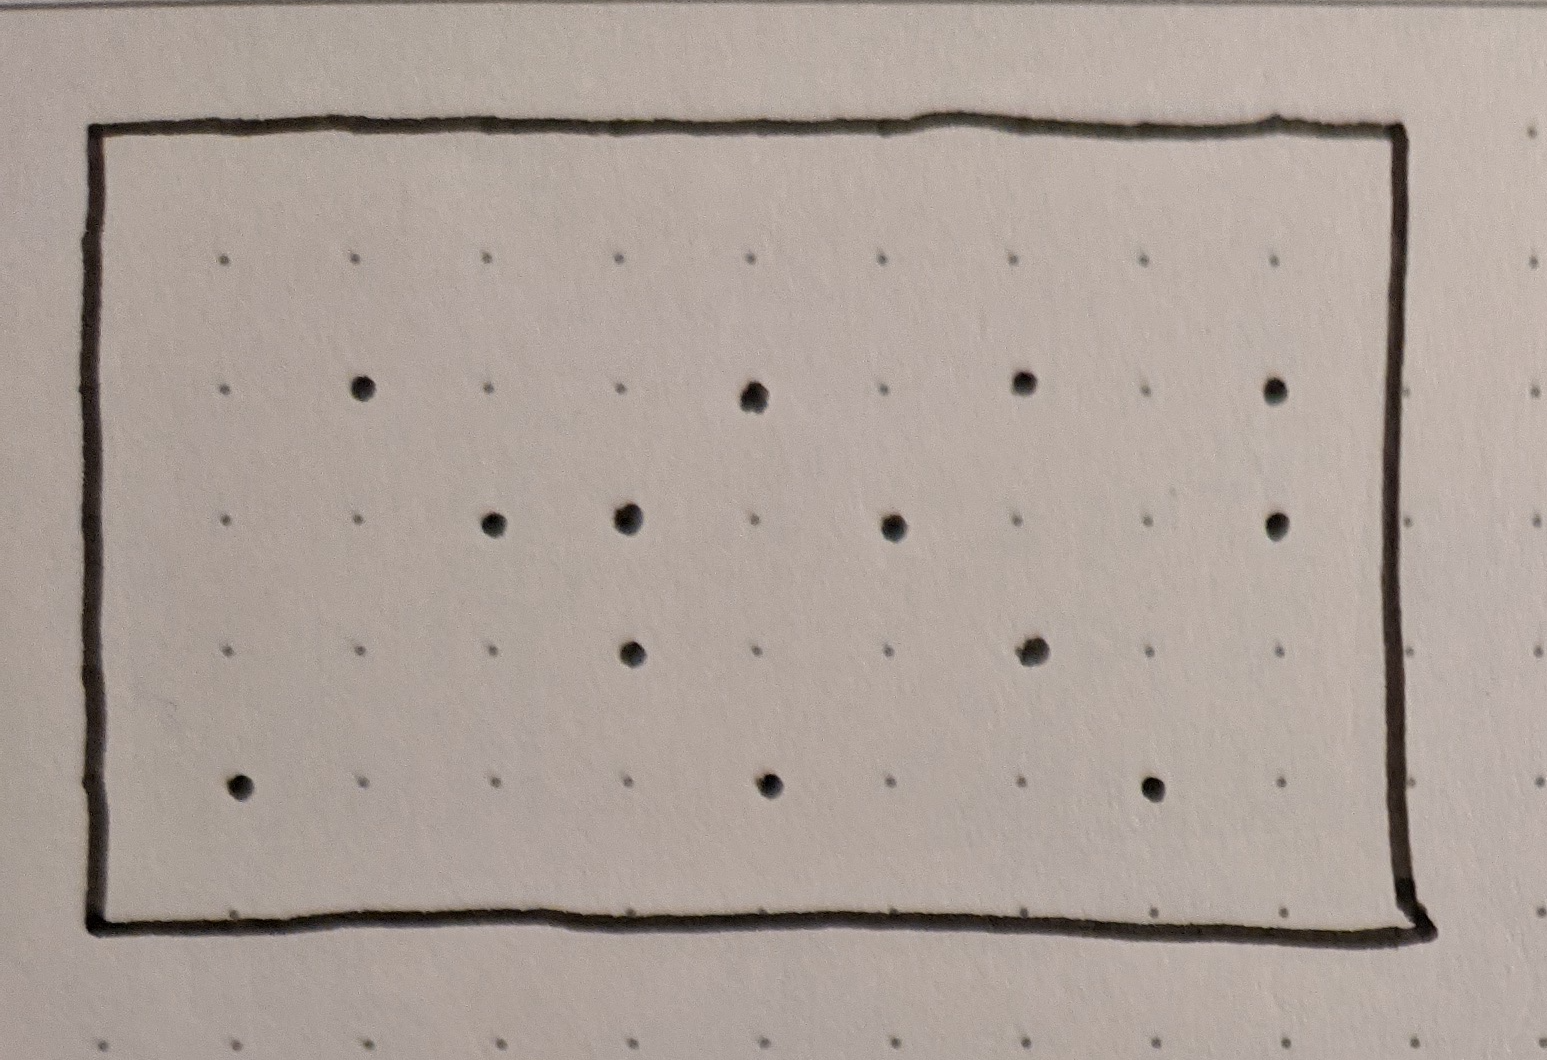
\includegraphics[width=0.3\textwidth]{figures/diagram1.png}}
%    \hspace{1em}
%    \subfloat[$\{s | s \in \termlang \wedge \phi(s)\}$ in red]{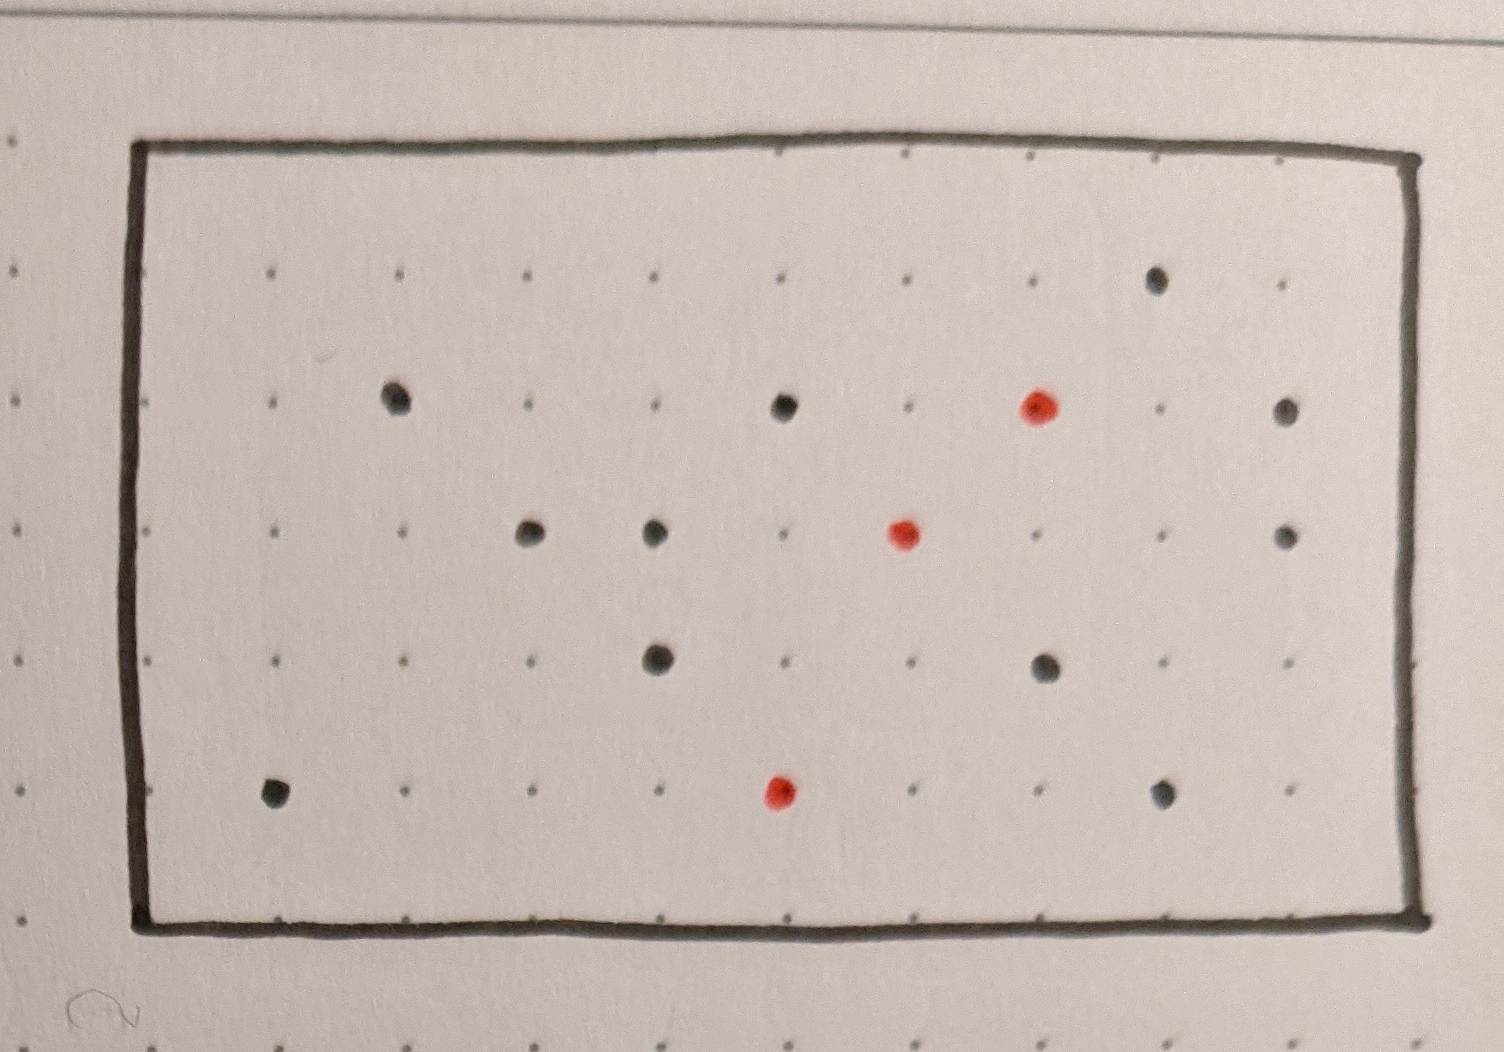
\includegraphics[width=0.3\textwidth]{figures/diagram2.png}}
%    \hspace{1em}
%    \subfloat[$\goallang$ in blue]{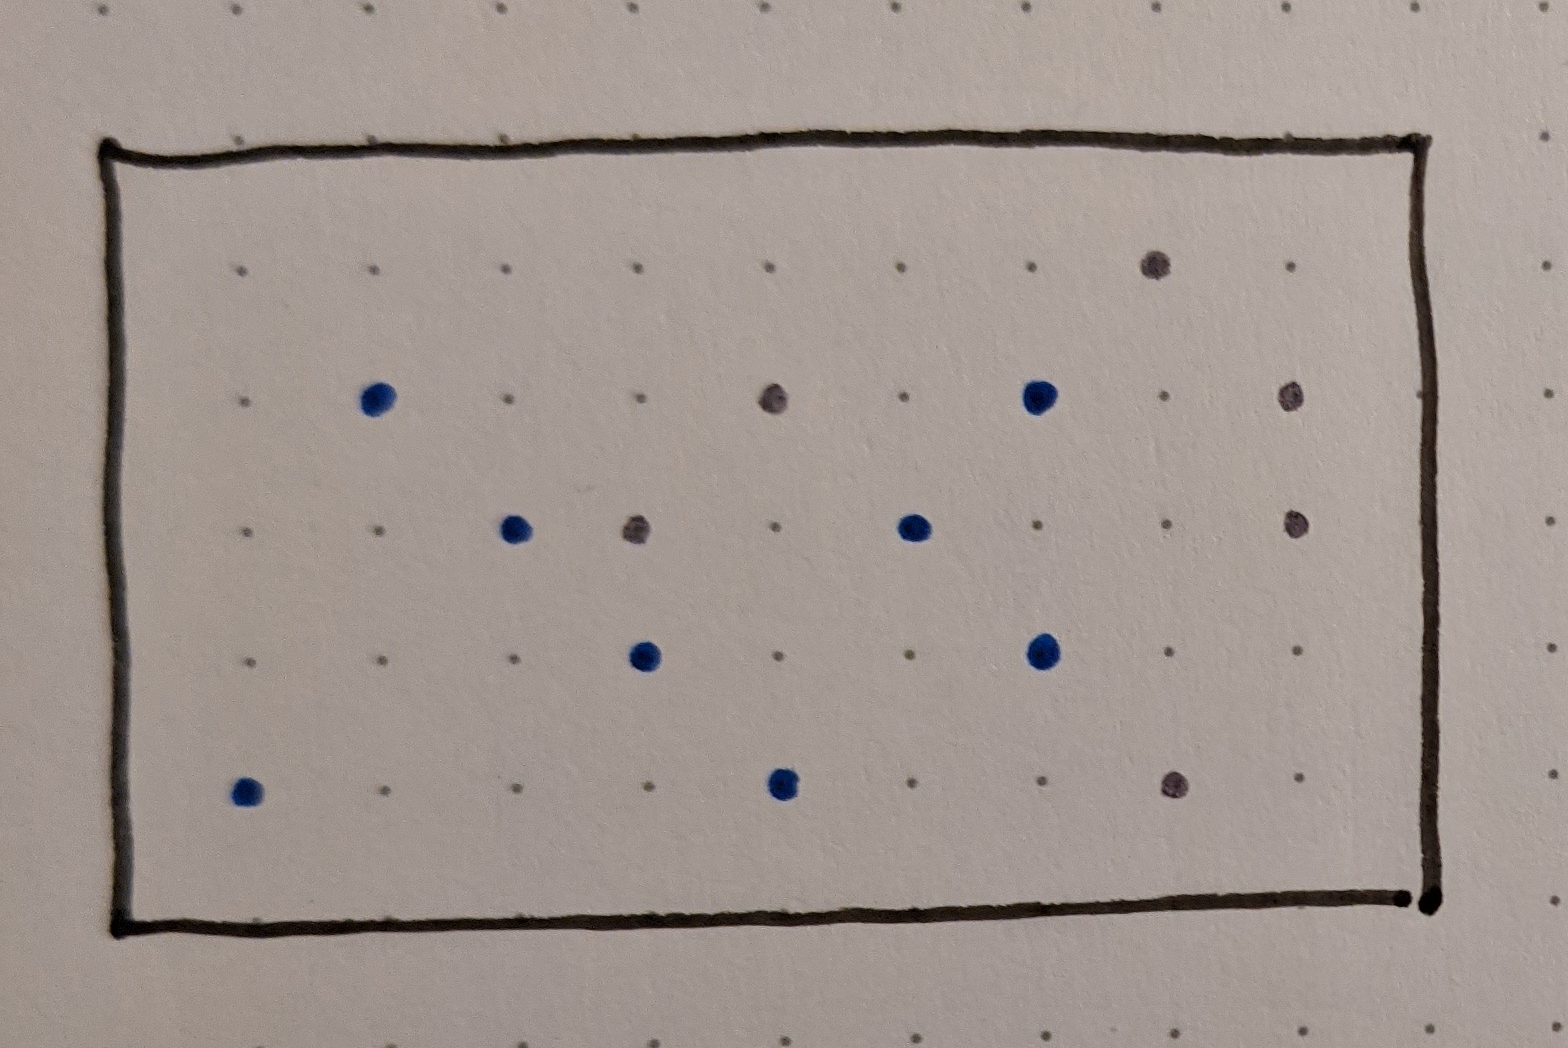
\includegraphics[width=0.3\textwidth]{diagram3.png}} \\
%    \subfloat[Undirected edges connect all $s, t$ st. $s =_e t$]{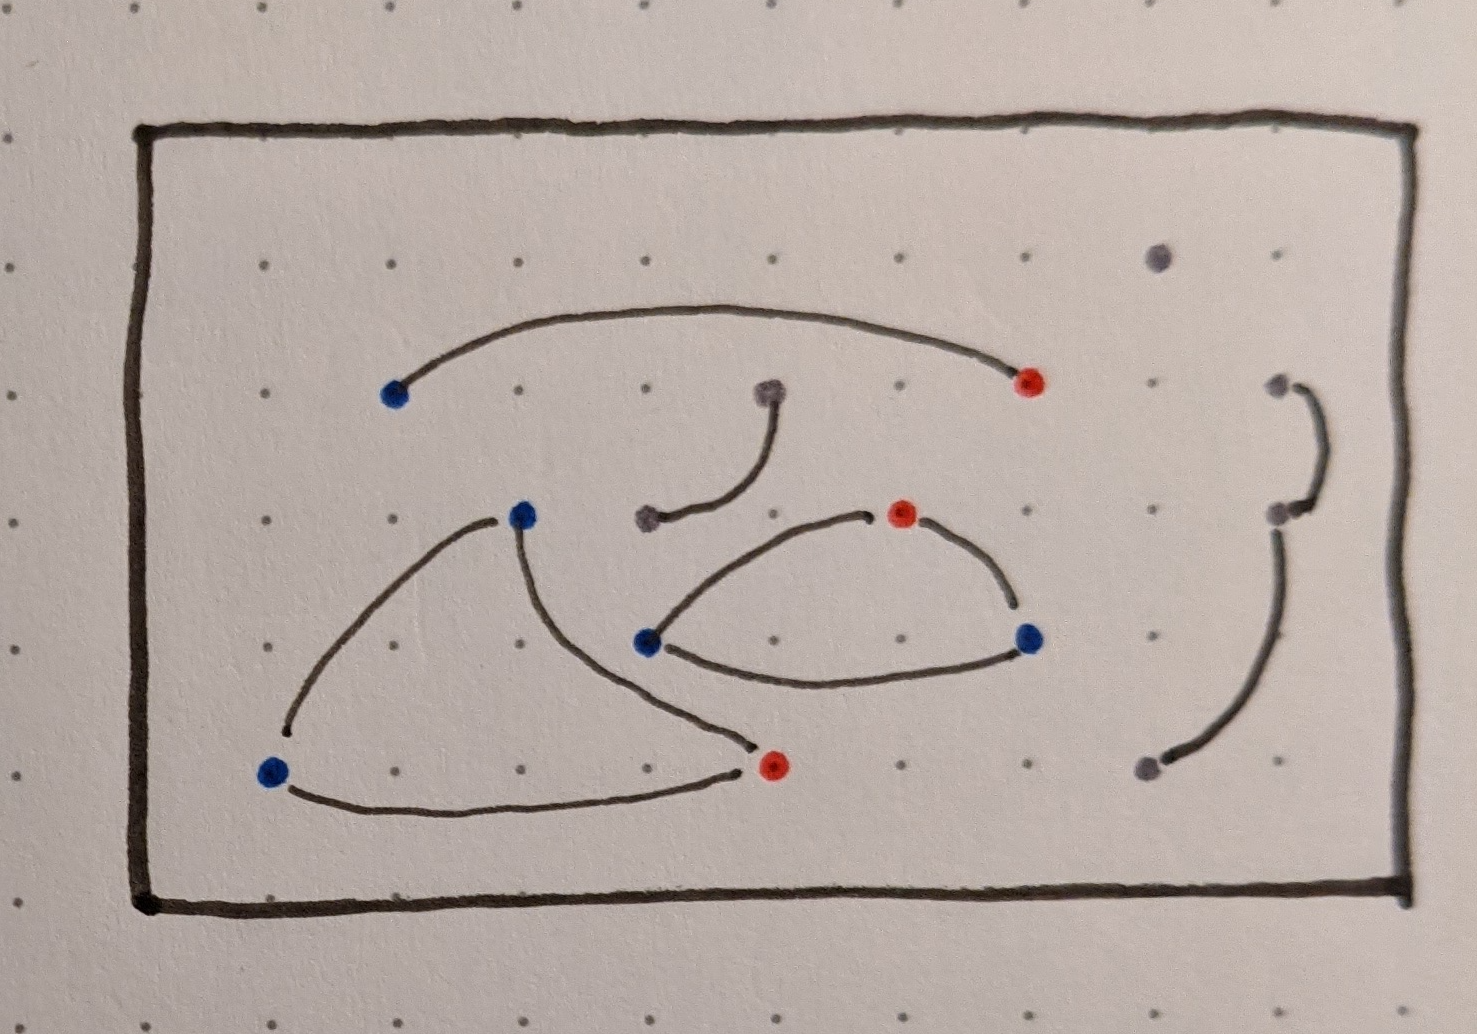
\includegraphics[width=0.3\textwidth]{figures/diagram4.png}}
%    \hspace{1em}
%    \subfloat[Directed edges connect all $s, t$ st. $s =_e t \wedge s > t$]{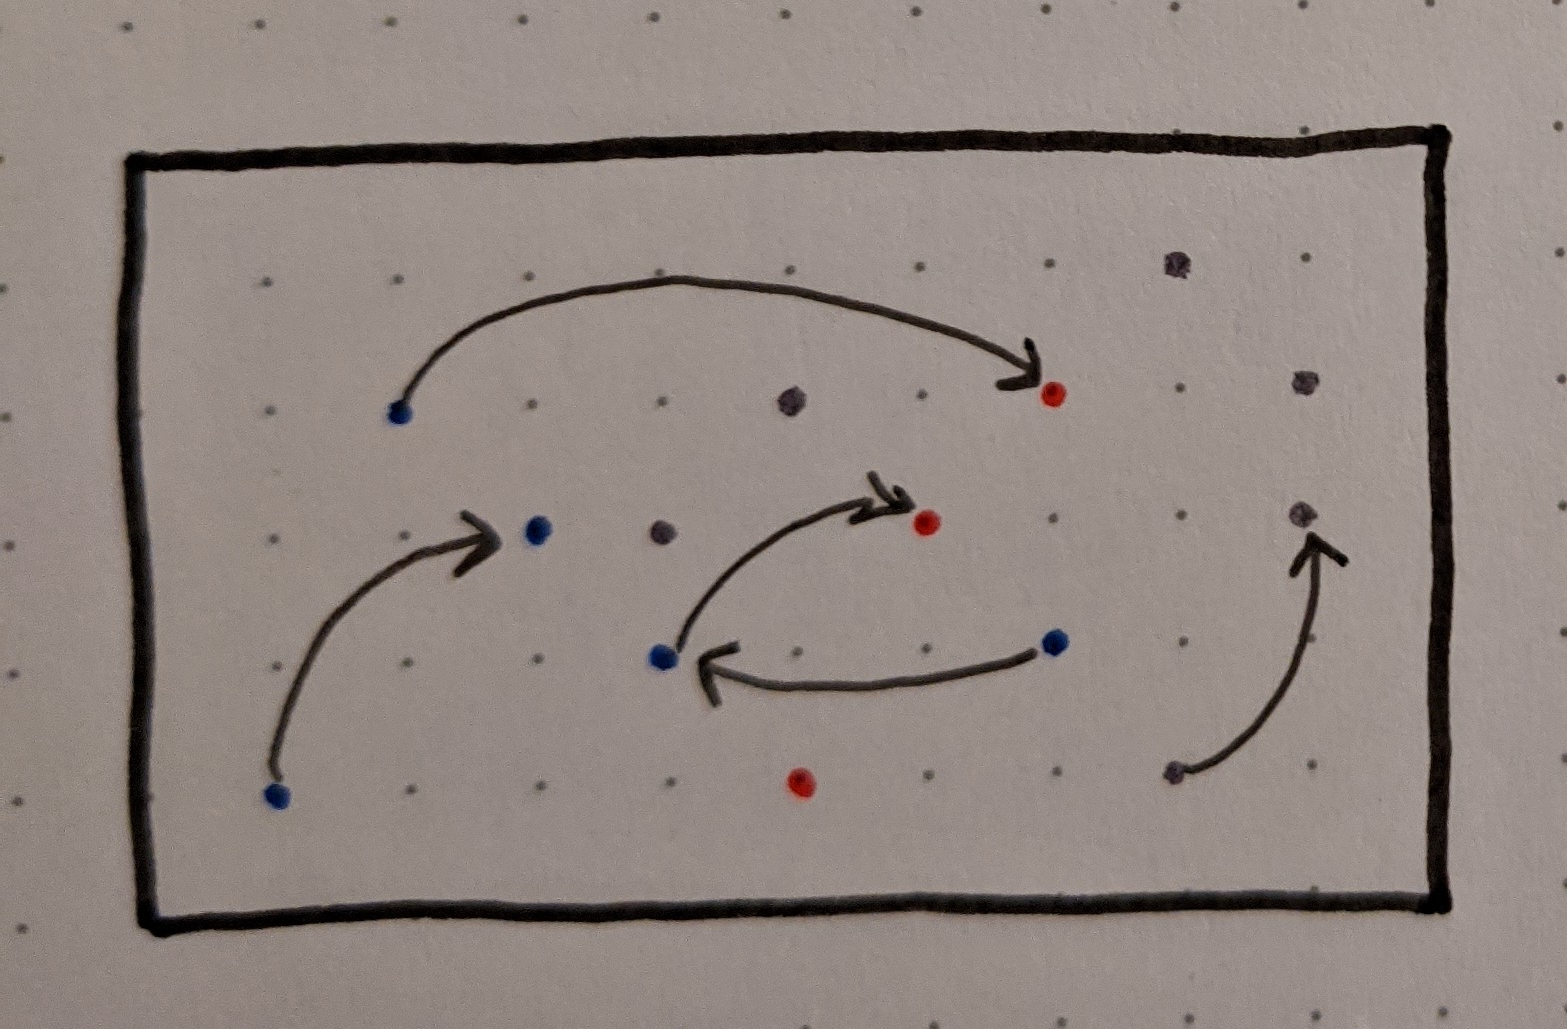
\includegraphics[width=0.3\textwidth]{figures/diagram5.png}}
%    \caption{Each dot in (a) represents a term in $\termlang$. In (b), each term in the goal state is drawn in red. In (c), all terms which are equivalent to a term in the goal state are drawn in blue. The goal of the term rewriting system is to rewrite all blue dots in (c) to a red dot in (b). In (d), undirected edges connect all pairs of terms that are semantically equivalent. In (e), those edges have been oriented with a reduction order. Given the specification $\forall (l \rewrites r) \in R \st l =_e \wedge l > r$, we can find a TRS $R$ by picking a finite subset of all the directed edges in (e).}
    \label{fig:termuniverse}
\end{figure}

First, we define the goal property that describes the underlying intention of the term rewriting system. Assume some language of terms $\termlang$, a semantic equivalence relation over those terms $=_e$, and a syntactic equivalence relation $=$. We write the goal property as a predicate function $\phi$ such that $\phi(s)$ is true if $s$ is in the goal state and false otherwise. We can thus write the domain of the term rewriting system as a language $\goallang \subseteq \termlang$, defined as

\[
\goallang = \{s | s \in \termlang \wedge (\exists t \in \termlang\;.\; s =_e t \wedge \phi(t))\}
\]

We want our term rewriting system to put every term in $\goallang$ into a form that satisfies our goal function $\phi$. It doesn't matter what the term rewriting system does to terms which are in $\termlang$ but not $\goallang$ so long as it obeys the semantics-preserving and termination properties.\footnote{We might prefer that the term rewriting system act on terms not in $\goallang$ as little as possible, but this is purely for performance reasons and can be set aside for now.}

As two running examples, let us consider two term rewriting systems that represent different aspects of the Halide simplifier TRS. As in the rest of this work, we assume that $\termlang$ is the Halide expression grammar. First, we consider a prover TRS, which tries to determine if an expression is equivalent to the booleans values true or false, or if its truth value is unknown. We state that the prover has a domain language $\goallang_P$ and a goal state function $\phi_P$ such that

\begin{align*}
    \goallang_P = \{s | s \in \termlang \wedge (s =_e \htrue \vee s =_e \hfalse)\} \\
    \phi_P(s) := s = \htrue \vee s = \hfalse
\end{align*}

The second example is a TRS that seeks to show that a given expression is monotonic. The goal function for this TRS is a bit more subtle. The Halide compiler's means of querying the monotonicity of an expression is sound but not complete: it walks the expression to see if it is in a syntactic form that can be recognized as monotonically increasing, monotonically decreasing, or constant. If it cannot recognize the expression as any of these three, it returns unknown. The job of the monotonic rewriter TRS is to put expressions into this syntactic form wherever possible. We say then that the domain language of the monotonic rewriter $\goallang_M$ is all terms $s$ in $\termlang$ where there exists some term $t$ such that $s =_e t$ and $t$ is in a syntactic form that can be recognized as monotonic or constant by the function $\texttt{is_monotonic}$ in the Halide codebase. The goal state function $\phi_M$ returns false when $\texttt{is_monotonic}$ returns unknown on an input term, and true otherwise.

We write $R(s)$ for the output of a term rewriting system $R$ on the input term $s$. Assume we use the means of assuring semantics preservation and termination as used above. Then, for an equivalence relation $=_e$ and a goal function $\phi$, we write that a specification for an ideal TRS $R$ thus:

\begin{align*}
\forall s \in \goallang \st \phi(R(s)) \wedge \\
\forall t \in \termlang \st t =_e R(t) \wedge R(t) \textrm{ terminates }
\end{align*}

Of course, since our theory is undecidable, the $\forall s \in \goallang \st \phi(R(s))$ portion of our specification is almost certainly unrealizable in the general case. Instead, we would like to encode a means of making progress towards this goal, rather than ruling out all TRSs that do not achieve it. We can think of this as a strategy for rewriting terms to be closer to the desired goal state. For example, imagine we started writing rules for the prover, and started with this pair:

\begin{align*}
    x = x \rewrites \htrue \\
    x + (y - y) \rewrites x
\end{align*}

We might note that the second rule is canceling like terms, and add many more rules that do the same. If we wanted to formally encode this strategy, we could do so using an order over terms, such that terms that satisfy the goal condition $\phi$ would be least elements in that order. In the case of the prover, the order could be to compare terms by their length; since the boolean constant $\htrue$ is of the shortest possible length in the Halide expression language, it is a least element of this order. Let us call such an order $\goalorder$ and add it as a condition to our specification:

\begin{align*}
\forall s \in \goallang \st \phi(R(s)) \wedge  s \geq_{\phi} R(s) \wedge \\
\forall t \in \termlang \st t =_e R(t) \wedge  R(t) \textrm{ terminates }
\end{align*}

As pictured in figure~\ref{fig:termuniverse}, the process of choosing rewrite rules for a ruleset is choosing edges from the graph (d) and orienting them. The goal order $\goalorder$ could be considered an order traversal from terms not in the goal state to terms that are. 

Now, assume we have been given some solution to our specification in the form of a term rewriting system $R$. How can we prove that it fulfills our criteria? In prior work, we proved that a term rewriting system was semantics-preserving ($\forall t \in \termlang \st t =_e R(t)$) and terminating ($\forall t \in \termlang \st R(t) \textrm{ terminates }$) by showing that those properties held over every rule in the ruleset. We can use a similar strategy here: if the goal order $\goalorder$ holds for every rule in $R$, then it must hold for all of $R$ as a whole.

\begin{assumption}
We can lower our requirement that the ruleset $R$ rewrite every term in $\goallang$ to the goal state to the requirement that every rule in $R$ rewrites terms to be closer to the goal state, as described by a goal order $\goalorder$.
\end{assumption}

% describe this more clearly: 
Requiring the goal order hold over every rule in $R$ will exclude some possible term rewriting systems for which the goal order would hold over the full system, just as requiring that the termination property hold over every rule in $R$ excludes some TRSs that are terminating. This is illustrated in figure~\ref{fig:termuniverse}; when we choose an order that turns the undirected edges in (d) to directed edges in (e), there are now some terms in $\goallang$ that are unable to reach a goal state. However, checking that this property holds over every rule can be done quickly and automatically. Just as with the termination guarantee, so long as every rule we add to a ruleset conforms to the goal order, we can add, delete, or permute the priority of rules without fear of losing our overall guarantee. This quick machine-checkable proof allows us to synthesize a TRS without human supervision.

In order for the goal order to hold over every term that may match and be rewritten by a rule, it must be a valid reduction order: well-founded, $\Sigma$-operation compatible, and closed under substitution (see~\cite{baader1999term}). Usefully, this means we do not need a separate termination order; since a goal order requires that each rewrite moves a term monotonically lower in the order, it also provides a termination guarantee.

We can now restate our term rewriting system specification like so:

\begin{align*}
    \forall s \in \goallang \st \phi(R(s)) \wedge \\
    \forall (l \rewrites r) \in R \st l =_e r \wedge l \goalorder r
\end{align*}

Since any term rewriting system we wish to synthesize will be semantics-preserving, the major decision we need to make in specifying a term rewriting system is to pick a goal order:

\begin{assumption}
We can effectively formalize the goal of a term rewriting system by choosing a \emph{goal order} over terms such that, for two terms $s$ and $t$ such that $s \goalorder t$ in this order, $t$ is assumed to be closer to the goal state.
\end{assumption}

Finding a goal order that encodes progress towards a goal state is a difficult task, and requires human intuition and ingenuity. Our work does not directly aid in this task, which is still up to the human author of the term rewriting system; however, our proposed synthesizer machinery can aid in experimenting with and selecting goal orders, as will be discussed in section~\ref{sec:proposedexperiments}.

\begin{table}[]
    \centering
    \begin{tabular}{|l|l|l|}
    \hline 
        TRS & Goal function $\phi$ & Goal order $>$ \\
        \hline 
        Prover &  $\phi(s)$ if $s$ is $\htrue$ or $\hfalse$ & $s > t$ if $t$ is shorter than $s$\\
        \hline
        Monotonic rewriter & $\phi(s) := \texttt{is_monotonic(s)}$ & $s > t$ if $s$ has more $\%$ ops \\
                 & & $s > t$ if $s$ has more constants \\
        \hline
    \end{tabular}
    \caption{Two term rewriting systems, goal functions that encode their intent, and goal orders that represent moving towards those goals}
    \label{tab:trsspecs}
\end{table}

As discussed above, the prover could adopt a strategy of making expressions shorter, with the aim of eventually being able to reduce them to the constants $\htrue$ or $\hfalse$. For the monotonic rewriter, one expression in the goal state is $x \cdot c_0$ where $c_0$ is a positive constant; the monotonicity checker recognizes this form as monotonically increasing. So, one possible strategy could be to move constants to the right side of an equation wherever possible. We may also want to employ sub-strategies: if the prover TRS contains the rule $x = x \rewrites \htrue$, we might choose a strategy of putting expressions into a kind of canonical form wherever possible, so we can rewrite an expression $e_1 = e_2$ into $e' = e'$ and then apply the identity rewrite rule. The simplifier reduction order, which was composed of several orders lexicographically, could be said to employ a series of sub-strategies in this way. See table~\ref{tab:trsspecs} for the prover and monotonic rewriter goal functions and some goal orders that approximate them.
 % check with Andrew about monotonic rewriter example

If we accept the assumption that a reduction order can encode the strategy of rewriting a term to be closer to our goal, we now have a specification that should hold for every individual rule we synthesize:

\[ \forall (l \rewrites r) \in R \st l =_e r \wedge l \goalorder r
\]

The set of possible rules made up of terms in the Halide expression language that conform to that spec is still infinitely large. The other part of our spec required that $\forall s \in \goallang \st \phi(R(s))$, but this is unrealizable. Instead we relax to a specification that could actually be checked; for example, we could fix a set $S$ of terms and write that our term rewriting system should:

\begin{align*}
    \forall s \in S \st \phi(R(s)) \wedge \\
    \forall (l \rewrites r) \in R \st l =_e r \wedge l \goalorder r
\end{align*}

Now we have a realizable synthesis procedure: we can synthesize rules $(l \rewrites r)$ such that $l =_e r \wedge l \goalorder r$, add them to $R$, and terminate when $\forall s \in S \st \phi(R(s))$ holds, as described in algorithm~\ref{algo:synthesis}. In practical cases, we may want to use other termination conditions, such as requiring that some fraction of $S$ can be solved. In our prior work, we did not check that the outputs of the synthesis-augmented simplifier brought previously unsolved terms to the goal state at all, but relied on a fairly complex goal order to produce a strengthened ruleset that was demonstrably more effective on our benchmarks.

Finally, we need a strategy for choosing which rule to add to growing ruleset at each step. As the space of potential rules is so large, even if term sizes are bounded, simply sampling at random may not be effective. Our synthesis pipeline defines a strategy for growing a ruleset so that it is able to rewrite more and more of $\goallang$, in a way that is of practical benefit to the compiler. In prior work, we gathered a corpus of expressions seen by the compiler in realistic circumstances and mined them for general patterns to form candidate LHS terms. We then attempted to synthesize RHSs for each candidate LHS term to form rules. We assert that this is an effective method of creating a ruleset is effective under realistic workloads.

\begin{assumption}
An effective heuristic for choosing candidate left-hand side terms for new rules is to gather expressions seen by the compiler under realistic circumstances and mine them for general patterns.
\end{assumption}

Note that when we gathered input expressions in prior work, we did not check to see if those expressions were in the TRS domain $\goallang$. Any means of checking membership in $\goallang$ is necessarily incomplete, so any ruleset learned from a checked input list would inherit the incompleteness of the checker. Also, note that we will want to rewrite subterms of expressions that are not themselves in $\goallang$: in the prover TRS, although all input expressions are boolean-valued, we will want to rewrite subterms of all possible types. For example, given the ruleset $R = \{x = x \rewrites \htrue, x + x \rewrites x \cdot 2\}$, we need the second rule that rewrites a numeric-valued expression so that we can rewrite $x + x = x \cdot 2$ to $\htrue$.

Given these three assumptions, we propose the synthesis pipeline in algorithm~\ref{algo:synthesis}. 

\subsection{The Halide variable solver}

The Halide simplifier was a fairly mature system, in production for over a year and consists of almost a thousand rules. The Halide variable solver, by contrast, is a much smaller system, currently implemented as a series of if statements rather than a formal term rewriting system, and consisting of the equivalent of less than a hundred rules. The simplifier's use cases were quite varied and complex, and the existing ruleset required a complex composite reduction order to cover their full purpose. The variable solver is much smaller and more focused and can be captured by much simpler reduction orders. With the variable solver, therefore, we have the opportunity to experiment with various reduction orders to find the one that fulfills the system's purpose best, and to synthesize a TRS entirely from scratch, rather than augment an existing system.

% synthesis pipeline: Rosette, encoding reduction order as metasketches, metasketch search order, etc
% discussion of different granularities of reduction order
% evaluation of various synth'd TRSs
